\chapter{Горизонты, уравнение состояния и энергия вакуума}

\section{Выделенная система отсчета, сверхсветовое удаление и горизонт}

Космический микроволновой фон действительно выделяет особую систему отсчета. В системе отсчета, в которой это излучение выглядит изотропным, окрестные галактики тоже в среднем покоятся. Если мы движемся сквозь фон, то фотоны в направлении вперед доплеровски смещаются к более высоким энергиям, а фотоны в обратном направлении — к более низким. Выделенная система отсчета — это та, в которой микроволновой фон выглядит изотропным; это также, в среднем, система отсчета, в которой покоятся окрестные галактики.

\begin{classroomqa}
\lecturetimestamp{00:00:25}
\audiencequestion{Зависит ли наблюдаемая длина волны космического излучения от движения наблюдателя и означает ли это существование выделенной системы отсчета?}
\lecturerresponse{Да. Движение сквозь микроволновой фон порождает доплеровскую анизотропию, так что существует выделенная космологическая система отсчета: та, в которой микроволновой фон выглядит изотропным. Это также, в среднем, система отсчета, в которой покоятся окрестные галактики.}
\end{classroomqa}

Второй вопрос касается скоростей удаления. Закон Хаббла утверждает, что достаточно далекие галактики удаляются согласно
\begin{equation}
v = H d .
\end{equation}
Для достаточно больших \(d\) эта скорость удаления превышает скорость света. Это не противоречит теории относительности, потому что запрет носит локальный характер: один объект не может пройти мимо другого прямо у нас перед глазами со скоростью, большей скорости света. Утверждение о далеких галактиках — это утверждение о геометрии между далеко разнесенными областями.

\begin{classroomqa}
\lecturetimestamp{00:04:48}
\audiencequestion{Могут ли две галактики иметь относительную скорость, большую \(c\)?}
\lecturerresponse{Да, если они достаточно далеко разнесены. Хаббловское удаление может превышать скорость света, не нарушая локальной теории относительности, а место, где скорость удаления достигает \(c\), — это горизонт.}
\end{classroomqa}

Когда скорость удаления достигает скорости света, сигналы, посланные к нам, в суммарном итоге больше не продвигаются к нам. Луч по-прежнему локально движется с предельной скоростью, но расстояние, которое ему нужно преодолеть, растет слишком быстро.

\begin{classroomqa}
\lecturetimestamp{00:07:03}
\audiencequestion{Разве световой луч, посланный в обратном направлении, все равно не будет идти к нам?}
\lecturerresponse{Локально будет, но пространство растет быстрее, чем луч способен это преодолеть. Луч движется с предельной скоростью относительно соседних точек, тогда как полное расстояние до нас продолжает увеличиваться.}
\end{classroomqa}

\section{Расширяющаяся метрика и аналогия с линией}

Полезная наглядная картина здесь одномерна. Представьте себе линию, состоящую из атомов. Если растягивать обычную материальную линию, она в конце концов порвется. Теперь изменим картину: всякий раз, когда соседние атомы слишком сильно раздвигаются, мы вставляем между ними еще один. Линия продолжает расти, но ее локальная структура не становится более разреженной.

\begin{figure}
\centering
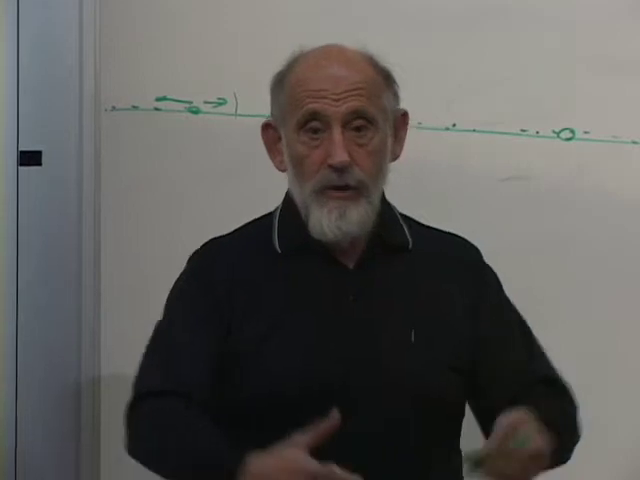
\includegraphics[width=0.60\textwidth]{lecture_04_figure_02.png}
\caption{Одномерная линия, используемая для наглядного изображения расширяющейся метрики.}
\end{figure}

В этой картине по-прежнему существует локальная предельная скорость сигнала, подобно тому как звук в обычной линии имеет предельную скорость. Правило локально: возмущение не может обогнать эту скорость относительно соседних точек. Тем не менее, если линия достаточно длинна и новые точки вставляются достаточно быстро, ее достаточно удаленные части удаляются так быстро, что сигнал никогда не сможет вернуться.

Поэтому специальнорелятивистский закон сложения скоростей — лишь часть картины. Он применим локально, когда наблюдатели проходят мимо друг друга в одной и той же точке. Для далеко разнесенных галактик в расширяющейся геометрии это не тот инструмент, который нужен.

\begin{classroomqa}
\lecturetimestamp{00:09:42}
\audiencequestion{Сохраняет ли в этой ситуации силу обычный релятивистский закон сложения скоростей?}
\lecturerresponse{Локально, в одной точке, да. Если наблюдатели последовательно проходят мимо друг друга, то действует обычное специальнорелятивистское правило. Но это не подходящий способ описывать удаление далеко разнесенных галактик со скоростью больше \(c\); здесь нужно вернуться к геометрии расширяющегося пространства.}
\end{classroomqa}

Та же картина дает простое объяснение красного смещения. Нарисуйте на линии волну. По мере расширения линии длина волны растет вместе с ней. В расширяющейся геометрии это не просто наглядный образ. Волновые уравнения в расширяющемся пространстве-времени действительно приводят к увеличению длины волны.

\begin{classroomqa}
\lecturetimestamp{00:14:42}
\audiencequestion{Является ли утверждение о том, что волна растягивается вместе со Вселенной, теоретическим, эмпирическим или и тем и другим?}
\lecturerresponse{Это теоретическое следствие распространения волн в расширяющемся пространстве-времени, и оно также подтверждается астрономическими наблюдениями.}
\end{classroomqa}

Эта картина — не резиновая лента. Резиновая лента при растяжении истончается, и тот, кто жил бы в такой среде, увидел бы изменение локальных свойств. Здесь же локальные свойства остаются теми же, тогда как глобальный масштаб расстояний растет.

\section{Последнее рассеяние и наблюдаемая Вселенная}

Горизонт — это место, где скорость удаления достигает скорости света. Поверхность последнего рассеяния лежит немного внутри него. Сигнал, испущенный с горизонта, растягивался бы неограниченно; излучение последнего рассеяния имеет огромное, но конечное красное смещение.

\begin{classroomqa}
\lecturetimestamp{00:17:53}
\audiencequestion{Какова связь между сверхсветовым удалением, поверхностью последнего рассеяния и наблюдаемой Вселенной?}
\lecturerresponse{Горизонт находится там, где скорость удаления достигает скорости света. Поверхность последнего рассеяния лежит немного внутри него, потому что ее красное смещение огромно, но конечно. Для практических целей она отмечает границу наблюдаемой Вселенной.}
\end{classroomqa}

Красное смещение излучения последнего рассеяния составляет приблизительно \(10^3\). Эта величина уже настолько велика, что поверхность последнего рассеяния для многих целей находится очень близко к горизонту. Наблюдаемая Вселенная — это та часть Вселенной, из которой свет может достичь нас.

На поздних стадиях расширение приближается к режиму, в котором доминирует энергия вакуума. Тогда величина Хаббла стремится к постоянной, горизонт стремится к фиксированному размеру, а и галактики, и микроволновое излучение постепенно исчезают из виду.

\begin{classroomqa}
\lecturetimestamp{00:22:43}
\audiencequestion{Поскольку \(H\) меняется со временем, меняется ли расстояние до горизонта и исчезнет ли в конце концов микроволновой фон?}
\lecturerresponse{На поздних стадиях \(H\) стремится к постоянной, так что горизонт стремится к фиксированному расстоянию. Микроволновой фон продолжает растягиваться, остывать и угасать. Далекие галактики тоже пересекают горизонт и исчезают из виду.}
\end{classroomqa}

Видимыми остаются только структуры, которые уже гравитационно связаны. Солнечная система не разлетается, и галактика не разлетается, но крупномасштабная Вселенная превращается в изолированный остров.

\section{Основное уравнение расширения и три компоненты}

Теперь основное уравнение расширения имеет вид
\begin{equation}
\left(\frac{\dot a}{a}\right)^2 = \frac{8\pi G}{3}\rho ,
\qquad c=1 .
\end{equation}
Здесь \(a(t)\) — масштабный фактор, а \(\rho\) — полная плотность энергии.

\begin{figure}
\centering
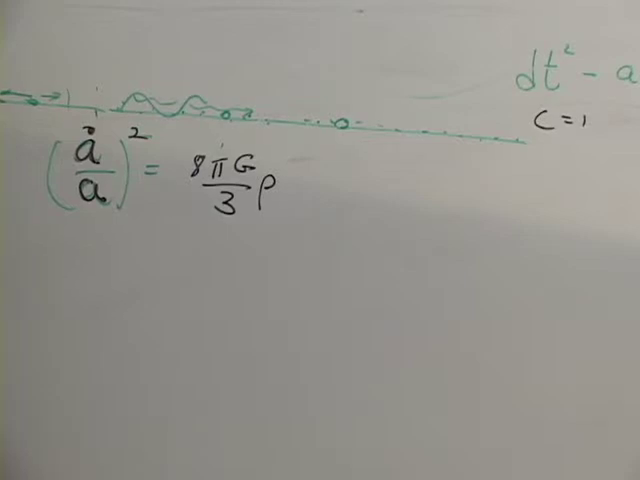
\includegraphics[width=0.74\textwidth]{lecture_04_figure_03.png}
\caption{Основное уравнение расширения и одномерная аналогия с линией.}
\end{figure}

Существуют три динамически важные компоненты.

Для материи,
\begin{equation}
\rho=\frac{\text{const.}}{a^3},
\qquad
a(t)\sim t^{2/3}.
\end{equation}
Это случай массивных объектов, участвующих в общем расширении и практически покоящихся в сопутствующей системе отсчета.

Для излучения,
\begin{equation}
\rho=\frac{\text{const.}}{a^4},
\qquad
a(t)\sim t^{1/2}.
\end{equation}
Дополнительная степень \(a\) обусловлена красным смещением каждого фотона по мере расширения Вселенной.

Есть также
\begin{equation}
\rho_0=\text{constant},
\end{equation}
энергия вакуума, также называемая темной энергией или, с точностью до общепринятых численных множителей, космологической постоянной. Эта компонента совсем не разрежается.

Следующий шаг — связать плотность энергии с давлением.

\section{Давление излучения и холодная материя}

Начнем с излучения. Рассмотрим одномерный ящик — просто отрезок длины \(L\), в котором фотоны движутся туда и обратно. В одном измерении сила и давление фактически совпадают.

Рассмотрим фотон с модулем импульса \(p\). При отражении от стенки его импульс изменяется на
\begin{equation}
\Delta p = 2p.
\end{equation}
Время между последовательными столкновениями с одной и той же стенкой равно
\begin{equation}
\Delta t = \frac{2L}{c}.
\end{equation}
Следовательно, средняя сила, действующая на стенку, равна
\begin{equation}
F=\frac{\Delta p}{\Delta t}=\frac{pc}{L}.
\end{equation}
Для фотона,
\begin{equation}
E=pc,
\end{equation}
так что
\begin{equation}
F=\frac{E}{L}.
\end{equation}
Энергия, деленная на длину, есть одномерная плотность энергии. В этом одномерном случае,
\begin{equation}
P=\rho .
\end{equation}

Для многих фотонов то же соотношение сохраняется и после усреднения. Полная сила — это просто полная энергия на единицу длины.

Теперь перейдём к трём измерениям. Если бы все фотоны двигались только вдоль одной оси, они оказывали бы давление на одну пару граней и не оказывали бы его на остальные. Это намеренно неверно, но сразу показывает, что нужно исправить. В изотропной ванне импульс распределён по всем направлениям. В среднем одна треть плотности энергии вносит вклад в каждую компоненту давления. Получаем
\begin{equation}
P=\frac{\rho}{3}.
\end{equation}

Для холодной материи ответ иной. Возьмём сопутствующий объём, небольшую область, движущуюся вместе с потоком Вселенной. Частицы внутри несут энергию, но если они покоятся относительно этого объёма, то не ударяются о его стенки. Поэтому давление равно
\begin{equation}
P=0.
\end{equation}

\begin{figure}
\centering
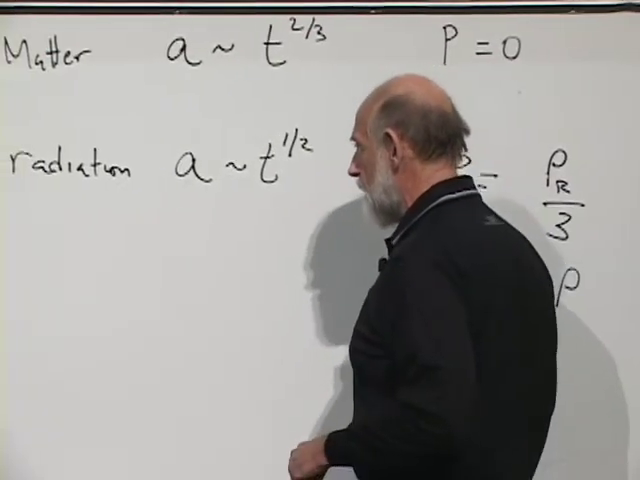
\includegraphics[width=0.74\textwidth]{lecture_04_figure_04.png}
\caption{Материя и излучение: \(a\sim t^{2/3}\), \(P=0\); \(a\sim t^{1/2}\), \(P=\rho/3\).}
\end{figure}

Итог на доске таков:
\begin{align}
\text{matter:}\qquad & a(t)\sim t^{2/3}, \qquad P=0,\\
\text{radiation:}\qquad & a(t)\sim t^{1/2}, \qquad P=\frac{\rho}{3}.
\end{align}

\begin{classroomqa}
\lecturetimestamp{00:54:27}
\audiencequestion{В расширяющейся Вселенной частицы ведь на самом деле разлетаются друг от друга?}
\lecturerresponse{Да, но рассуждение о давлении применяется к бесконечно малому сопутствующему объёму. На этом локальном масштабе термодинамическое рассуждение по-прежнему работает.}
\end{classroomqa}

\section{Уравнение состояния}

Предполагается, что давление пропорционально плотности энергии,
\begin{equation}
P=w\rho .
\end{equation}
На доске тот же параметр записан как \(\omega\). Для двух основных случаев
\begin{equation}
w=0 \quad \text{for cold matter},
\qquad
w=\frac{1}{3} \quad \text{for radiation}.
\end{equation}

Возможны и промежуточные случаи. Значения между \(0\) и \(1/3\) описывают вещество, которое не является ни полностью холодным, ни полностью релятивистским. Упомянутый здесь пример — тёплая тёмная материя.

\begin{figure}
\centering
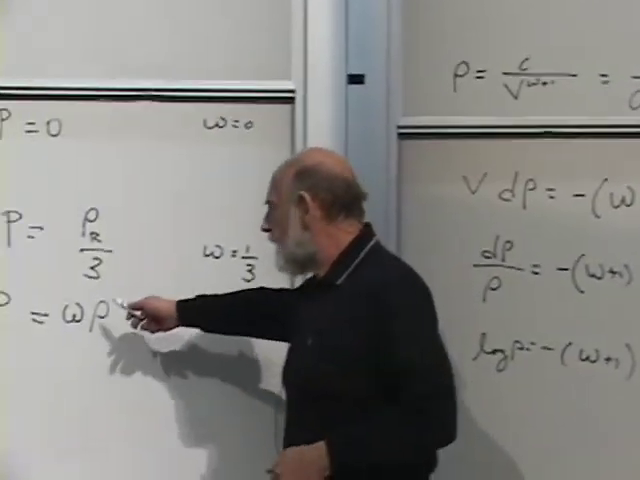
\includegraphics[width=0.74\textwidth]{lecture_04_figure_05.png}
\caption{Уравнение состояния \(P=\omega\rho\) и рассуждение о масштабировании плотности.}
\end{figure}

Следующий вопрос состоит в том, определяет ли \(w\) зависимость \(\rho\) от \(a\). Ответ следует из термодинамического тождества.

Возьмём ящик объёма \(V\). Если его содержимое оказывает давление \(P\), то при увеличении объёма ящика на \(dV\) работа, совершаемая над стенками, равна
\begin{equation}
dE=-P\,dV.
\end{equation}
Теперь запишем энергию в виде
\begin{equation}
E=\rho V.
\end{equation}
Её дифференциал равен
\begin{equation}
dE=\rho\,dV+V\,d\rho .
\end{equation}
Приравнивая эти два выражения, получаем
\begin{equation}
\rho\,dV+V\,d\rho=-P\,dV,
\end{equation}
или
\begin{equation}
V\,d\rho=-(\rho+P)\,dV.
\end{equation}
Используя \(P=w\rho\),
\begin{equation}
V\,d\rho=-(1+w)\rho\,dV.
\end{equation}
Разделим на \(\rho V\):
\begin{equation}
\frac{d\rho}{\rho}=-(1+w)\frac{dV}{V}.
\end{equation}
Интегрируя, получаем
\begin{equation}
\rho \propto V^{-(1+w)}.
\end{equation}
Для сопутствующего космологического объёма
\begin{equation}
V\propto a^3,
\end{equation}
и, следовательно,
\begin{equation}
\rho \propto a^{-3(1+w)}.
\end{equation}

Сразу получаются уже рассмотренные случаи:
\begin{align}
w=0 &\Longrightarrow \rho \propto a^{-3},\\
w=\frac{1}{3} &\Longrightarrow \rho \propto a^{-4}.
\end{align}

Вот почему важен \(w\). Как только известна \(\rho(a)\), её можно подставить обратно в уравнение Фридмана. Затем пробуют степенной закон \(a\sim t^\alpha\) и определяют, как расширяется Вселенная при таком уравнении состояния.

\section{Вакуумная энергия и отрицательное давление}

Один особый случай ведёт себя иначе:
\begin{equation}
w=-1.
\end{equation}
Тогда
\begin{equation}
1+w=0,
\end{equation}
так что показатель обращается в нуль и
\begin{equation}
\rho=\rho_0=\text{constant}.
\end{equation}
Соответствующее давление равно
\begin{equation}
P=-\rho .
\end{equation}

Отрицательное давление само по себе не является чем-то загадочным. Положительное давление толкает стенки ящика наружу. Отрицательное тянет их внутрь. Это натяжение. Обыденный пример — растянутая резинка: она запасает положительную энергию, но стягивает свои концы.

Подставим постоянную плотность \(\rho_0\) в уравнение Фридмана:
\begin{equation}
\left(\frac{\dot a}{a}\right)^2=\frac{8\pi G}{3}\rho_0.
\end{equation}
Правая часть — просто число, поэтому
\begin{equation}
\frac{\dot a}{a}=\sqrt{\frac{8\pi G}{3}\rho_0}.
\end{equation}
Это особый случай, в котором величина Хаббла действительно постоянна. Уравнение можно записать в виде
\begin{equation}
\dot a=\sqrt{\frac{8\pi G}{3}\rho_0}\,a,
\end{equation}
и его решение имеет вид
\begin{equation}
a(t)\propto \exp\!\left(\sqrt{\frac{8\pi G}{3}\rho_0}\,t\right).
\end{equation}

Это экспоненциальное расширение. Характерным масштабом времени здесь является время увеличения в \(e\) раз, а не время удвоения, и использованная здесь грубая оценка даёт величину порядка возраста Вселенной. Вакуумная энергия и космологическая постоянная — это одна и та же физическая составляющая, если не считать исторически сложившихся численных соглашений.

\begin{classroomqa}
\lecturetimestamp{01:27:16}
\audiencequestion{Если вакуумная энергия вызывает экспоненциальное расширение, разве в конце концов всё не будет разорвано?}
\lecturerresponse{Не обязательно. Связанные системы могут этому сопротивляться. Галактика, Солнечная система или атом не обязаны быть разорваны, тогда как достаточно большие и разрежённые структуры действительно участвуют в расширении и в конце концов расходятся.}
\end{classroomqa}

\begin{classroomqa}
\lecturetimestamp{01:31:43}
\audiencequestion{Есть ли что-нибудь интересное в отрицательном знаке, когда берут квадратный корень из уравнения Фридмана?}
\lecturerresponse{Да. Квадратный корень даёт две ветви. Одна — расширяющееся решение, а другая — обращённое по времени сжимающееся решение. Сами уравнения допускают обе.}
\end{classroomqa}

\section{Три эры и наблюдаемая история расширения}

Присутствуют все три компоненты, и масштабируются они по-разному:
\begin{equation}
\begin{aligned}
\rho_{\text{radiation}}&\propto a^{-4},\\
\rho_{\text{matter}}&\propto a^{-3},\\
\rho_0&=\text{constant}.
\end{aligned}
\end{equation}
Отсюда сразу следуют три эры.

При очень малых \(a\) доминирует излучение. Позже доминирует материя. При достаточно больших \(a\) доминирует вакуумная энергия. Соответствующие законы расширения имеют вид
\begin{equation}
a(t)\sim t^{1/2},
\qquad
a(t)\sim t^{2/3},
\qquad
a(t)\sim e^{Ht}.
\end{equation}

Приведённые здесь грубые времена таковы: примерно через \(10^4\) лет излучение уступает место материи. Позже, примерно через \(10^5\) лет, Вселенная становится прозрачной. Переход от доминирования материи к ускоренному расширению происходит намного позже, спустя несколько миллиардов лет, примерно на середине космической истории в используемой здесь оценке по порядку величины.

Как восстанавливают эту историю? Будущее мы видеть не можем, но прошлое можем. Смотреть на большие расстояния значит смотреть в более раннее время. Наблюдая далёкие галактики, измеряя, как их движение связано с расстоянием, и восстанавливая величину Хаббла как функцию времени запаздывания, восстанавливают временную зависимость масштабного фактора. Эра доминирования излучения слишком ранняя, чтобы её можно было непосредственно увидеть в обычной галактической астрономии, но эра доминирования материи и переход к доминированию вакуума видны на восстановленной кривой.

\section{Последнее рассеяние в далёком будущем}

Микроволновая картина неба в будущем — не то же самое, что исчезновение галактик за горизонтом. Излучение, которое мы видим в более поздние времена, приходит от более далёкого вещества, так что эффект состоит скорее в том, что мы заглядываем всё глубже и видим всё более холодное излучение, а не в том, что наблюдаем, как одни и те же атомы просто удаляются.

\begin{classroomqa}
\lecturetimestamp{01:48:07}
\audiencequestion{Если поверхность последнего рассеяния уходит в горизонт, то это то же самое, что галактики уходят за горизонт?}
\lecturerresponse{Нет. Более позднее излучение приходит не от тех же атомов, что излучение, которое мы видим сейчас. Оно приходит от атомов, которые находились дальше, так что это похоже на всё более глубокий взгляд во Вселенную, тогда как само излучение выглядит всё более холодным.}
\end{classroomqa}

\section{Кривизна, картина Большого схлопывания и горизонт на поздних временах}

До этого момента член с кривизной опускался. Если восстановить его, получаем
\begin{equation}
\left(\frac{\dot a}{a}\right)^2
=
\frac{8\pi G}{3}\rho
-
\frac{K}{a^2}.
\end{equation}
Численно этот член кажется малым, но концептуально он важен. На более старом ньютоновском языке он различает случаи положительной, нулевой и отрицательной полной энергии. На релятивистском языке он различает пространственные геометрии.

До того как к вакуумной энергии стали относиться всерьёз, часто представляли себе Вселенную, в которой доминирует материя и расширение в конце концов сменится сжатием. Отсюда возникала старая картина Большого схлопывания: расширение после Большого взрыва, а затем повторное сжатие. Математика по-прежнему верна, но больше не выглядит описанием нашей Вселенной.

\begin{classroomqa}
\lecturetimestamp{01:53:51}
\audiencequestion{Связана ли эта вакуумная энергия с квантовой энергией вакуума?}
\lecturerresponse{Да, или по крайней мере считается, что связана.}
\end{classroomqa}

Приблизительный сегодняшний состав таков:
\begin{equation}
\frac{\rho_0}{\rho_{\text{total}}}\sim 0.7,
\qquad
\frac{\rho_{\text{matter}}}{\rho_{\text{total}}}\sim 0.3.
\end{equation}
Внутри этой компоненты материи вклад светящейся материи составляет около \(0.05\), а тёмной материи — около \(0.25\) от общей плотности. Излучением сегодня можно пренебречь. Тёмная и светящаяся материя масштабируются одинаково, поэтому их отношение остаётся фиксированным, хотя относительная доля материи, излучения и вакуума меняется от эры к эре.

В пределе доминирования вакуума
\begin{equation}
H=\sqrt{\frac{8\pi G}{3}\rho_0}.
\end{equation}
Тогда закон Хаббла принимает вид
\begin{equation}
v=Hd.
\end{equation}
Горизонт определяется условием \(v=1\), поэтому его расстояние равно
\begin{equation}
d_H=\frac{1}{H}
=
\frac{1}{\sqrt{8\pi G\rho_0/3}}.
\end{equation}
Приведённая здесь грубая величина составляет примерно от \(10\) до \(12\) миллиардов световых лет.

Важно поведение на поздних временах. Как только расширение становится экспоненциальным, расстояние до горизонта фиксируется. Галактики продолжают пересекать его и исчезать по мере того, как их красный сдвиг всё растёт. Микроволновой фон тоже уходит в красный сдвиг. В очень далёком будущем видимыми останутся только близкие гравитационно связанные структуры, и Вселенная будет выглядеть как изолированный остров.

\section{Геометрия по поверхности последнего рассеяния}

Наконец, геометрию можно проверить по поверхности последнего рассеяния. Предположим, что расстояние до этой поверхности известно. Предположим также, что там можно выделить неоднородность, физический размер которой известен достаточно хорошо. Тогда можно сопоставить этот размер и это расстояние с наблюдаемым угловым размером.

В плоском пространстве угол совпадает с евклидовым. В пространстве положительной кривизны он казался бы больше; в пространстве отрицательной кривизны — меньше. Аналогия — с обычными геодезическими измерениями: взять объект известного размера на известном расстоянии и сравнить измеренный угол с предсказанием евклидовой геометрии.

\begin{classroomqa}
\lecturetimestamp{02:08:09}
\audiencequestion{Какой можно привести пример объекта там, размер которого нам известен?}
\lecturerresponse{Крупнейшие неоднородности микроволнового фона. Мы полагаем, что знаем их размер по тому, сколько времени заняла их эволюция, и по скорости звука.}
\end{classroomqa}

Здесь существенны крупнейшие неоднородности микроволнового фона. Их наблюдаемый угловой размер оказывается согласованным с евклидовой геометрией с точностью до нескольких процентов. На этом основании пространство представляется плоским.

\section{Измеренное значение \(w\) и заключительный вопрос}

Теперь ясна важность \(w\) для наблюдений. Если астрономы сообщают, что \(w\) очень близко к \(-1\), то они тем самым говорят, что компонента вакуумной энергии почти постоянна. Именно это здесь и утверждается.

Это не означает, что общая теория относительности вынуждает \(w\) быть в точности \(-1\). Суть здесь эмпирическая. В лекции кратко отмечается, что более радикальные возможности в принципе не исключены, но веские основания имеются именно в пользу случая почти постоянной вакуумной энергии.

\begin{classroomqa}
\lecturetimestamp{02:11:04}
\audiencequestion{При вычислении плотности для вещества и для излучения мы предполагали, что энергия постоянна, а затем подстраивали масштабный фактор, чтобы вывести формулу? И если это верно для первых двух случаев, то что происходит в случае вакуумной энергии, где плотность остается постоянной?}
\lecturerresponse{Нет. Я не предполагал, что она постоянна. Мы использовали то, что изменение энергии равно \(-P\,dV\). Для воображаемого сопутствующего ящика, движущегося вместе с расширением, на стенках совершается работа, и этим объясняется изменение энергии. Случай вакуумной энергии ставит вопрос по-иному, и заключительное замечание здесь состоит в том, что язык закона сохранения энергии в космологии мало что говорит, потому что полная энергия Вселенной равна нулю.}
\end{classroomqa}